% ------------------------------------------------------------------------
% Poster: Modelo de Poster para eventos de Lic. Inform.  
% 
% Template por Francisco Reinaldo 
%		(https://orcid.org/0000-0001-6161-6755)
%		(http://lattes.cnpq.br/7401534350061823)
% ------------------------------------------------------------------------
% Agradecimentos a Overleaf pela oportunidade 
% ------------------------------------------------------------------------

\def\footer#1{\def\insertfooter{#1}}
\documentclass[final]{beamer}

\usepackage[scale=1.150]{beamerposter}
\usetheme{MUWposter} 

%\logo{\pgfputat{\pgfxy(-13,108.5)}{\pgfbox[center,base]{\includegraphics[width=18cm]{logo_UTFPR.jpg}}}}  

\usepackage{multicol}
\usepackage{array}
%The following two are column definitions for the aknowledgements section
\newcolumntype{L}{>{\arraybackslash}m{22cm}}
\newcolumntype{S}{>{\arraybackslash}m{5cm}}
\usepackage{pgf}
%\usepackage{helvet}
\usepackage{mathtools}
\usepackage{amsmath, amsthm, amssymb, amsfonts}
\usepackage{exscale}
\usepackage{xcolor}
\usepackage{ushort}
\usepackage{setspace}
\usepackage{transparent}
\usepackage[square,numbers]{natbib}
\usepackage{url}
\bibliographystyle{abbrvnat}
\renewcommand{\vec}[1]{\ushort{#1}}
\renewcommand{\vec}[1]{\mathbf{#1}}
\definecolor{greenMUW}{RGB}{60,191,174}
\definecolor{blueMUW}{RGB}{17,29,79}
\definecolor{skinMUW}{RGB}{254,228,217}
\definecolor{hellblauMUW}{RGB}{95,180,229}
\usepackage{xcolor}
\usepackage{graphicx}
%-----------------------------------------------
%  START Set the colors
%  Uncomment to apply colors you want to use.
%-----------------------------------------------
\colorlet{themecolor}{greenMUW}
\usebackgroundtemplate{
\includegraphics[width=90cm,height=120cm]{MUW_green}}


%-----------------------------------------------
%  START Set the width of the columns
%-----------------------------------------------
\setlength{\paperwidth}{90cm} % A0 width: 46.8in
\setlength{\paperheight}{120cm} % A0 height: 33.1in
\newlength{\sepmargin}
\newlength{\sepwid}
\newlength{\onecolwid}
\newlength{\twocolwid}
\newlength{\threecolwid}
\usepackage{caption}
\captionsetup[figure]{labelformat=empty}%

% The following measures are used for 2 columns
\setlength{\sepmargin}{0.055\paperwidth} % Separation width (white space) between columns
\setlength{\sepwid}{0.03\paperwidth} % Separation width (white space) between columns
\setlength{\onecolwid}{0.425\paperwidth} % Width of one column
%\setlength{\twocolwid}{0.6\paperwidth} % Width of two columns

%-----------------------------------------------------------
% The following measures are used for 3 columns
%\setlength{\sepmargin}{0.06\paperwidth} % Separation width (white space) between columns
%\setlength{\sepwid}{0.02\paperwidth} % Separation width (white space) between columns
%\setlength{\onecolwid}{0.28\paperwidth} % Width of one column
%\setlength{\twocolwid}{0.58\paperwidth} % Width of two columns
%\setlength{\threecolwid}{0.88\paperwidth} % Width of three columns
%\setlength{\columnsep}{30pt}

%-----------------------------------------------
%  END Set the width of the columns
%-----------------------------------------------


%------------------------
\setbeamertemplate{title}[left]
\setbeamertemplate{frametitle}[default][left]
%\setmainfont{Georgia}

\title{Deep Optimal Transport for Domain Adaptation Application to Vehicle Re-Identification}
%small{Projeto  RED n.6, homologado, Edital 32/2014 PROGRAD - Produção de Recursos Educacionais Digitais]}\\}

\author{\textbf{Yujin CHO, Israfel SALAZAR}} % Author(s)

\institute{M1 E3A @ Université Paris-Saclay. Paris, France} % Institution(s)
%------------------------

\usepackage[absolute,overlay]{textpos}
  \setlength{\TPHorizModule}{1mm}
  \setlength{\TPVertModule}{1mm}

\begin{document}
%verificar width=10cm,height=10cm,keepaspectratio
\begin{textblock}{20}(580,30)

\includegraphics[scale=0.9]{images/evryyyy.png}
\end{textblock}

\begin{textblock}{20}(700,30)
\transparent{1}
\includegraphics[width=16cm]{images/logoParisSaclay.png}
\end{textblock}

%\begin{textblock}{20}(500,32.5)
%\includegraphics[width=10cm]{selos_ge2017.pdf}
%\end{textblock}

  \addtobeamertemplate{block end}{}{\vspace*{1ex}} % White space under blocks
  \addtobeamertemplate{block alerted end}{}{\vspace*{0ex}} % White space under highlighted (alert) blocks
  \setlength{\belowcaptionskip}{2ex} % White space under figures
  \setlength\belowdisplayshortskip{1ex} % White space under equations
  

\begin{frame}[t] 
\begin{columns}[t] 
\begin{column}{\sepmargin}\end{column}
\begin{column}{\onecolwid} % The first column
\vspace{1em}
  \begin{block}{Introduction}
\textbf{Vehicle re-Identification is the task of finding the queried vehicle from the non-overlapping cameras, and the goal of attribute recognition is to predict the presence of a set of attributes from an image. It is part of smart city concept that aims to improve the quality of life of city dwellers by making the city more adaptive and efficient, using new technologies that are based on an ecosystem of objects and services.}
\end{block}
          
\begin{block}{Define the Problem}
\textbf{For each vehicle, there are big intra-class difference and learning all class distributions would need a huge amount of data. We proposed to train a model using only the front and rear view of vehicles, our hypotheses was that using domain adaptation we would be able to obtain good results in the vehicle re-identification problem for different distributed datasets.}

\begin{figure}
\vspace*{0.2cm}
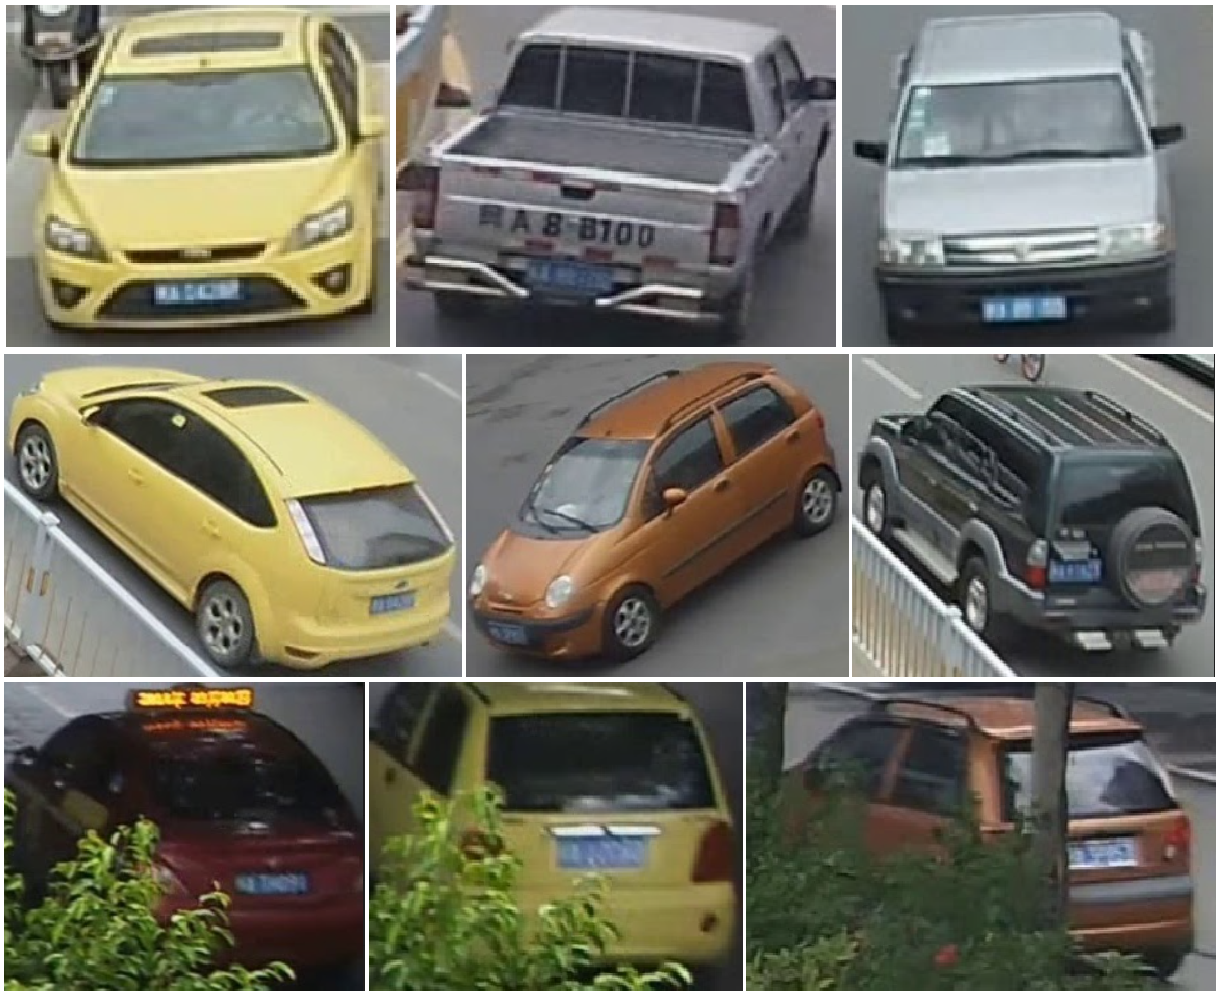
\includegraphics[width=0.45\linewidth]{images/compil.png}
\end{figure}

\end{block}    
          
\begin{block}{Objectives}
\textbf{With a limited amount of data using a dataset created using few cameras (view of vehicles), implement the domain adaptation algorithm using optimal transport to improve accuracy of model in unseen and with different distribution cameras ).}
\end{block}

\begin{block}{What is optimal transport?}

\begin{minipage}{0.4\textwidth}
    \begin{figure}[H]
        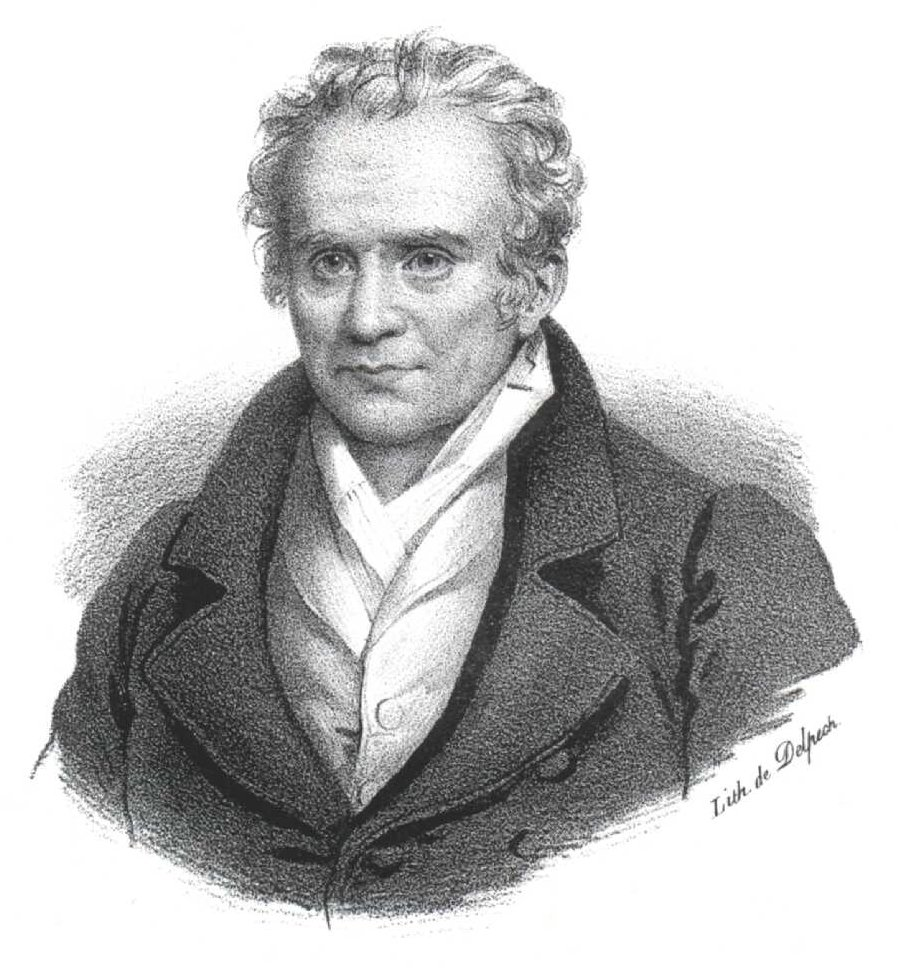
\includegraphics[width=0.7\linewidth]{images/gm.jpg}
        \caption{Gaspard Monge}
    \end{figure}
\end{minipage} \hfill
\begin{minipage}{0.6\textwidth}
    \textbf{Optimal Transport problem allows us to compare probability distributions in a geometrically manner. We search for the most economical way, for example in distance, to transport the distribution of a set of data to another using the geometry of the feature space.}
\end{minipage}

\begin{figure}
    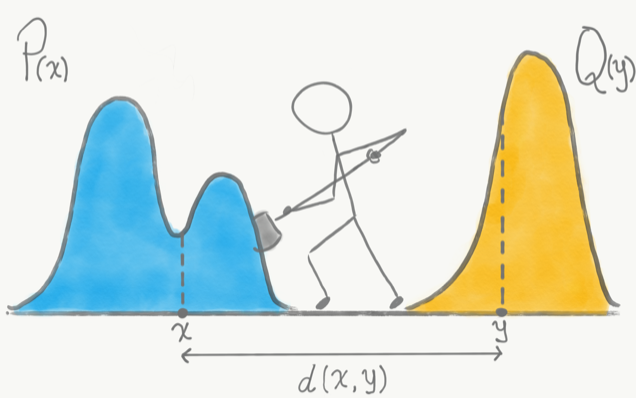
\includegraphics[width=0.45\linewidth]{images/OT_shovel.png}
    \caption{Earth mover distance}
\end{figure}

\textbf{The earth mover's distance (EMD) is a measure of the distance between two probability distributions over a region D (Also known as the Wasserstein metric). The EMD is the minimum cost to move from distribution P(x) to Q(y)}
\end{block}

\end{column} %fim coluna 1    
\begin{column}{\sepwid}\end{column} % separador coluna
\begin{column}{\onecolwid} %The second column
\vspace{1em}
 \begin{block}{DeepJDOT Implementation}

\begin{figure}
    \vspace*{0.2cm}
    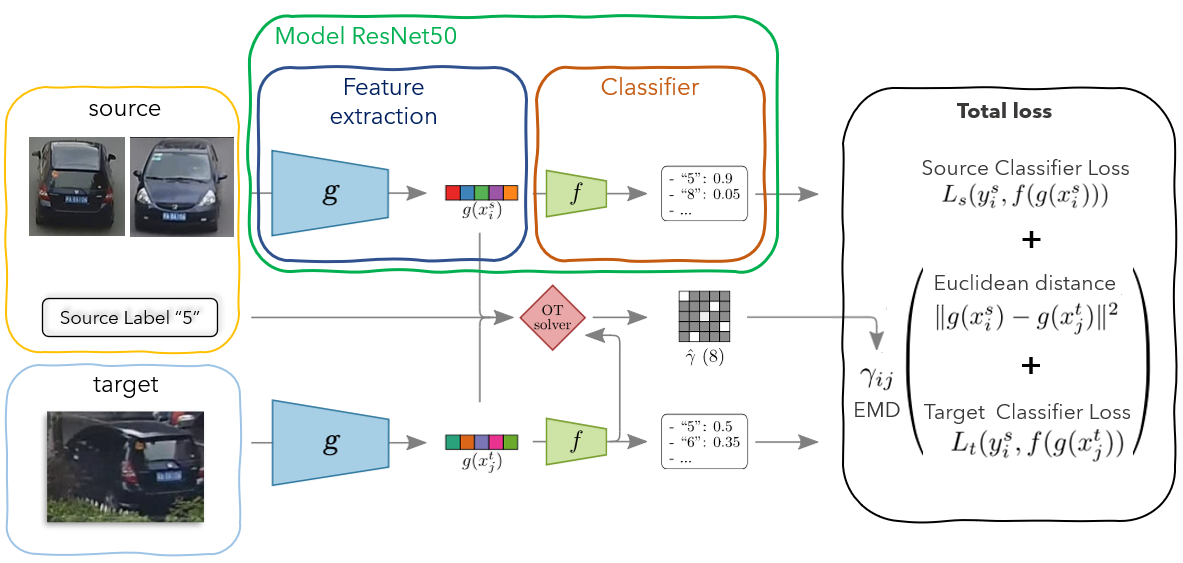
\includegraphics[width=1\linewidth]{images/jdotnet.PNG}
    \caption{DeepJDOT architecture}
\end{figure}
 
 \textbf{DeepJDOT uses a CNN model to solve the problem of different distribution between source and target. We used a ResNet50 model (pre-trained on ImageNet) divided in 2 parts (g = feature extractor and f = classifier).\\ }
 
\begin{figure}
    \vspace*{1cm}
    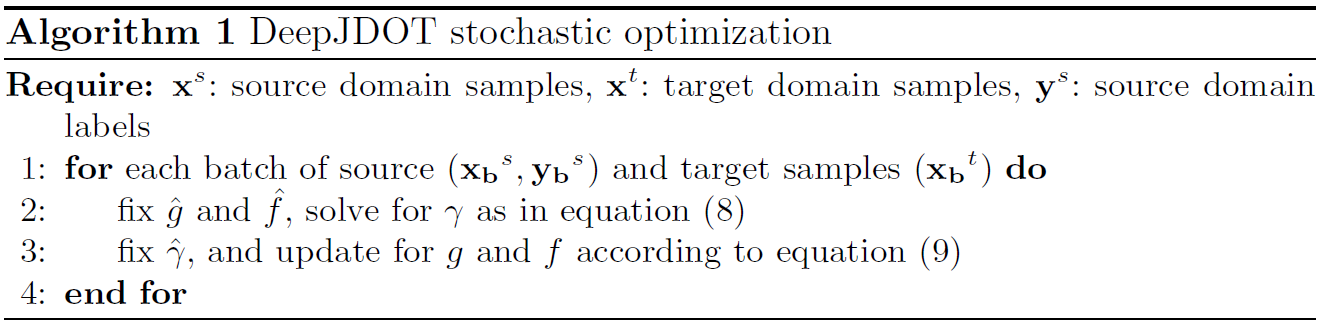
\includegraphics[width=1\linewidth]{images/jdotalgo.PNG}
    \caption{DeepJDOT algorithm}
\end{figure}
\textbf{Cross Entropy loss is used to back-propagate classifier estimations. The cost function $\gamma$ is computed between the features of source and target, then it's minimized by using EMD. The total loss is then computed and we update the models by backpropagation.}
 
 \end{block}
               
\begin{block}{Expected results}
 
% \begin{center}
%     \begin{tabular}{||c|c|c||} 
%     \hline
%     ResNet50 & Accuracy Source & Accuracy target\\ [0.5ex] 
%     \hline\hline
%     trained on source & $95.6\%$ & $40\%$ \\ 
%     \hline
%     trained w/ DeepJDOT & ? & ? \\
%     \hline
%    \end{tabular}
%\end{center}
    \textbf{Model trained with DeepJDOT method should perform better on target data than model trained only on source data}
\begin{figure}
    %\vspace*{1cm}
    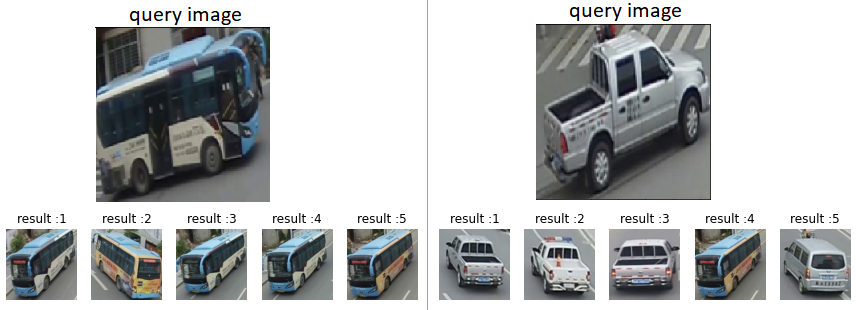
\includegraphics[width=1\linewidth]{images/resultJDOT.PNG}
    \caption{Top5 result closest result in source dataset}
\end{figure}
 
 \end{block} 
 
\begin{block}{Difficulties of implementation}
    \begin{itemize}
      \item \textbf{Dataset management to split source and training datas}
      \item \textbf{DeepJDOT training stability : best accuracy ~25\% }
      \item \textbf{Implementation of EMD (Optimal transport solver)}
      \item \textbf{Hyperparamters Searching and Fine tuning}
    \end{itemize}
\end{block} 
 
\end{column}%fim coluna 2
\begin{column}{\sepmargin} \end{column}
\end{columns} 
\end{frame} 
	
\end{document}


